\section{Evaluation}
\label{sec:evaluation}

\subsection{Implementation}
\label{sec:impl}

We implement all three WAL systems on top of CCBench~\cite{tanabe2020ccbench},
a concurrency-control benchmarking framework with minimal functionality
for protocol analysis.  The underlying engine is an ERMIA-style
multi-version store with snapshot isolation and SSN validation, using
Masstree as the index and \texttt{mimalloc} as the allocator.  The code
is written in C++20 and compiled with GCC at the \texttt{-O3}
optimization level.  Our implementation is publicly
available.\footnote{The source code is available in our public
repository for reproduction.}

A key methodological point is that Single WAL, P-WAL, and Ayame are
implemented in the \emph{same} binary and selected at run time by
environment flags (\texttt{CCBENCH\_WAL\_MODE} and
\texttt{CCBENCH\_WAL\_DURABLE\_MODE}).  The concurrency-control engine,
the index, the workload generator, and the pre-commit path are therefore
identical across the three systems; only the WAL durability path differs.
Single WAL appends to one shared log stream under a global latch and
synchronizes it per commit.  P-WAL gives each worker a private stream
and synchronizes it per commit, acknowledging through a global durable
prefix.  Ayame uses the worker/flusher/committer pipeline of
Section~\ref{sec:design} with dependency-closed acknowledgment.  Each WAL
record carries the key, value, storage identifier, and operation type of
a write, terminated by a commit record.  Read-only WAL skipping is
enabled for all three systems; once a transaction is known to be
read-only it produces no WAL record, and Ayame additionally takes a
read-only snapshot-isolation fast path that skips durability-frontier
collection.

Following the worker/flusher/committer separation of
Section~\ref{sec:design}, Ayame offloads durability to background
threads: it uses 1, 1, 1, 2, 4, and 7 flusher threads for 1, 2, 4, 8,
16, and 32 worker threads, respectively, and one committer thread in all
configurations.  The x-axis of our worker-scaling experiments is the
number of transaction worker threads; at 32 workers Ayame therefore runs
40 active threads (32 workers, 7 flushers, and one committer).

\subsection{Experimental Configuration}
\label{sec:config}

\subsubsection{Environment}
\label{sec:env}

Experiments were conducted on a server with two sockets of Intel(R)
Xeon(R) Gold 5418N CPUs.  Each socket had 24 physical cores with two
hardware threads per core, for 48 physical and 96 logical cores in
total, organized as two NUMA nodes.  Each core had a 48\,KiB private L1d
cache and a 2\,MiB private L2 cache, and each socket shared a 45\,MiB L3
cache.  The DRAM capacity was 256\,GB.  The machine ran Ubuntu 22.04.5
LTS (Linux kernel 5.15), and WAL files were placed on a locally attached
SSD formatted with ext4.  Worker threads were pinned to distinct logical
cores with \texttt{sched\_setaffinity}.

\subsubsection{Benchmark and Workloads}
\label{sec:workloads}

All experiments used the Yahoo! Cloud Serving Benchmark
(YCSB)~\cite{cooper2010ycsb}.  We evaluated three representative workloads:
YCSB-A (50\% read, 50\% update), YCSB-B (95\% read, 5\% update), and
YCSB-C (read-only).  These workloads exercise the WAL along a spectrum
from update-heavy to read-only and are widely used to evaluate
concurrency-control protocols.  Each transaction issued a fixed number
of ten operations over a database of 100{,}000 records with 4-byte
values, and keys were drawn from a uniform distribution.

\begin{table}[tb]
  \centering
  \caption{Default parameter settings.}
  \label{tab:params}
  \small
  \begin{tabular}{llr}
    \hline
    Type & Parameter & Setting \\
    \hline
    DB & \#records & 100{,}000 \\
       & value size & 4\,B \\
       & key distribution & uniform \\
    \hline
    TX & \#operations & 10 \\
       & read ratio & 50 / 95 / 100\,\% \\
    \hline
    Run & worker threads & 1,2,4,8,16,32 \\
        & measurement time & 5\,s \\
        & repeats & 5 \\
    \hline
    Ayame & flush group size [commits] & 16 \\
          & flush interval & 50\,$\mu$s \\
          & max pending acks & 65{,}536 \\
    \hline
  \end{tabular}
\end{table}

\subsubsection{Metric}
\label{sec:metric}

The primary metric is \emph{durable-acknowledgment throughput}: the
number of transactions acknowledged as durable to the client, divided by
the measurement time.  All systems are measured at the same stop
barrier, and acknowledgments drained during shutdown are excluded.  For
the worker-wait systems (Single WAL and P-WAL) a logical commit and a
durable acknowledgment coincide, so the metric has the same meaning
across the three systems.  We additionally report the p99 durable
acknowledgment latency and the number of pending (not-yet-acknowledged)
durable commits.

\subsection{Results}
\label{sec:results}

We evaluate Ayame using the worker-thread sweep of
Table~\ref{tab:params}.  At 32 worker threads on YCSB-A, Single
WAL achieves 9K durable acknowledgments per second and P-WAL achieves 54K,
whereas Ayame achieves 253K durable acknowledgments per second.  On YCSB-B,
Single WAL achieves 24K and P-WAL achieves 195K, whereas Ayame achieves 470K
durable acknowledgments per second.  These results correspond to 4.7$\times$
and 2.4$\times$ improvements over P-WAL on YCSB-A and YCSB-B, respectively.
Ayame also keeps the number of pending durable commits small at 32 worker
threads: 201 pending commits on YCSB-A and 68 pending commits on YCSB-B.
At 4 and 8 worker threads on YCSB-A, however, pending durable commits reach the
configured backpressure bound and the p99 acknowledgment latency rises into the
hundred-millisecond range (Figures~\ref{fig:ycsbabc-worker-latency}
and~\ref{fig:ycsbabc-worker-pending}), before recovering at 16 and 32 worker
threads as additional flusher threads are provisioned.

Figure~\ref{fig:ycsbabc-worker-throughput} shows the worker-thread comparison.
The results show that Ayame improves update and mixed read-write workloads,
where durable logging is still required on every update commit.  We also evaluate YCSB-C,
where all transactions are read-only and WAL records are skipped.  In this case,
durability work largely disappears; after using the same binary and a read-only
empty-frontier fast path, Single WAL, P-WAL, and Ayame perform similarly at 32
worker threads.  We therefore use YCSB-C as a sanity check for read-only
bookkeeping overhead rather than as evidence of WAL persistence performance.

\begin{figure*}[!tbp]
  \centering
  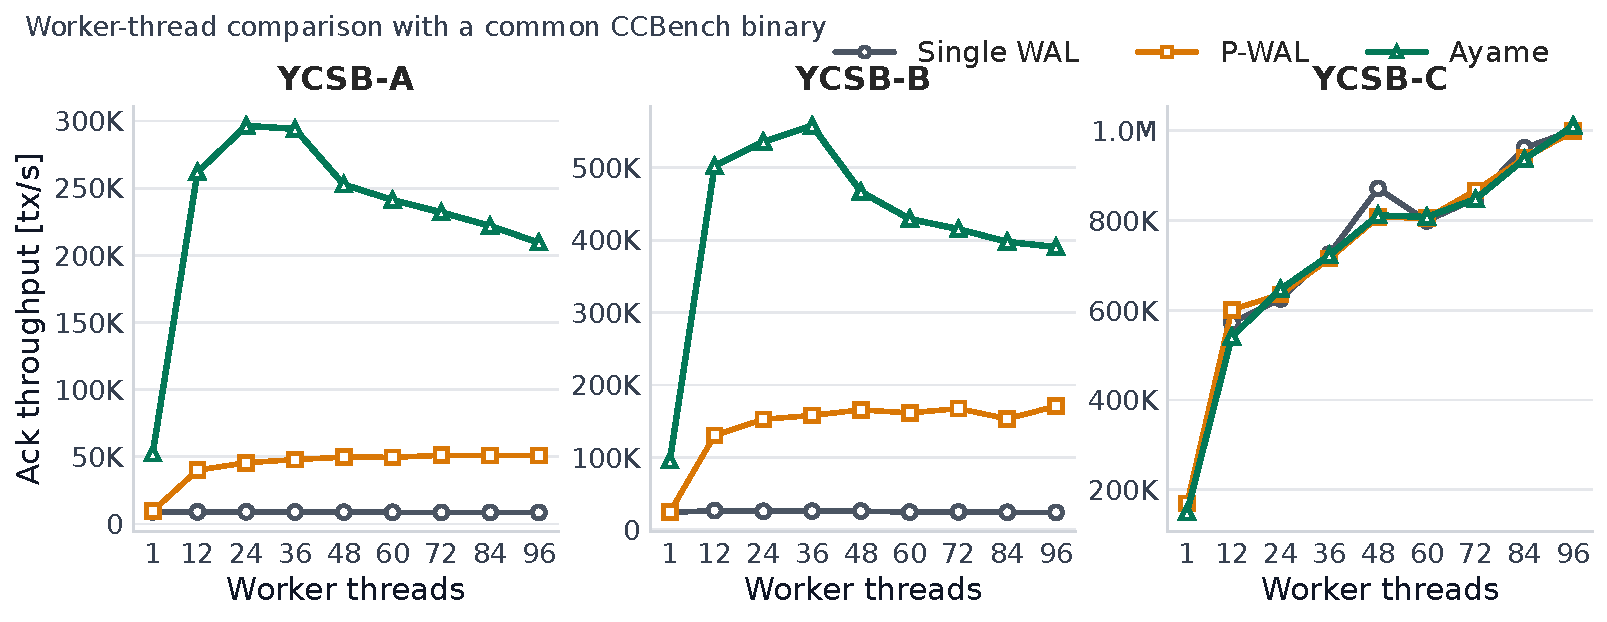
\includegraphics[width=\linewidth]{figures/fig_ycsbabc_worker_threads_throughput.pdf}
  \caption{
  Durable-acknowledgment throughput by transaction worker threads.
  Ayame improves update and mixed read-write workloads by combining parallel
  WAL logging, dependency-closed durable acknowledgment, and timestamp-integrated
  logical ordering.
  }
  \label{fig:ycsbabc-worker-throughput}
\end{figure*}

Ayame's timestamp integration is primarily a design simplification: it removes
duplicated logical ordering between concurrency control and WAL durability by
reusing ERMIA's commit timestamp as the logical recovery order.  We do not rely
on timestamp integration alone as a direct throughput optimization; the main
performance effect comes from parallel logging, dependency-closed durable
acknowledgment, and separating workers from durable-wait processing.

\begin{figure*}[!tbp]
  \centering
  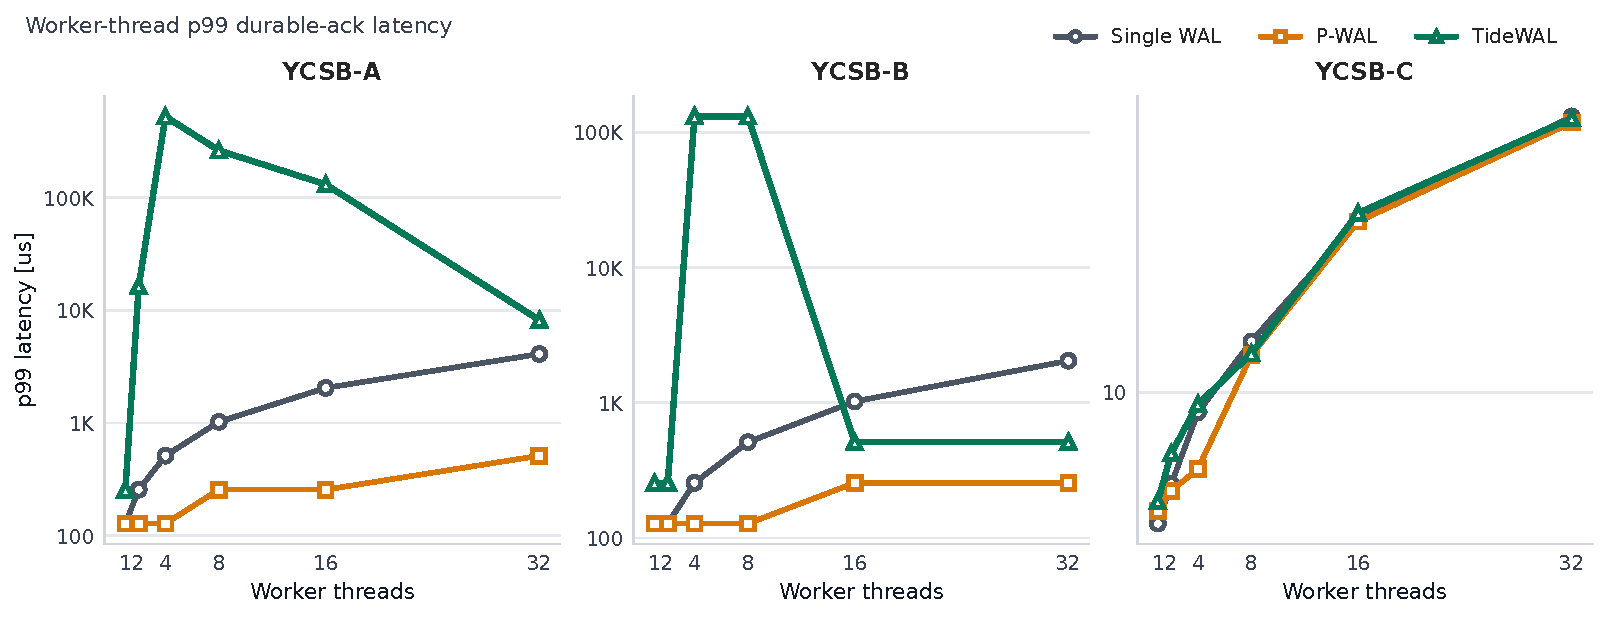
\includegraphics[width=\linewidth]{figures/fig_ycsbabc_worker_threads_latency.pdf}
  \caption{
  P99 durable-acknowledgment latency by transaction worker threads.
  }
  \label{fig:ycsbabc-worker-latency}
\end{figure*}

\begin{figure*}[!tbp]
  \centering
  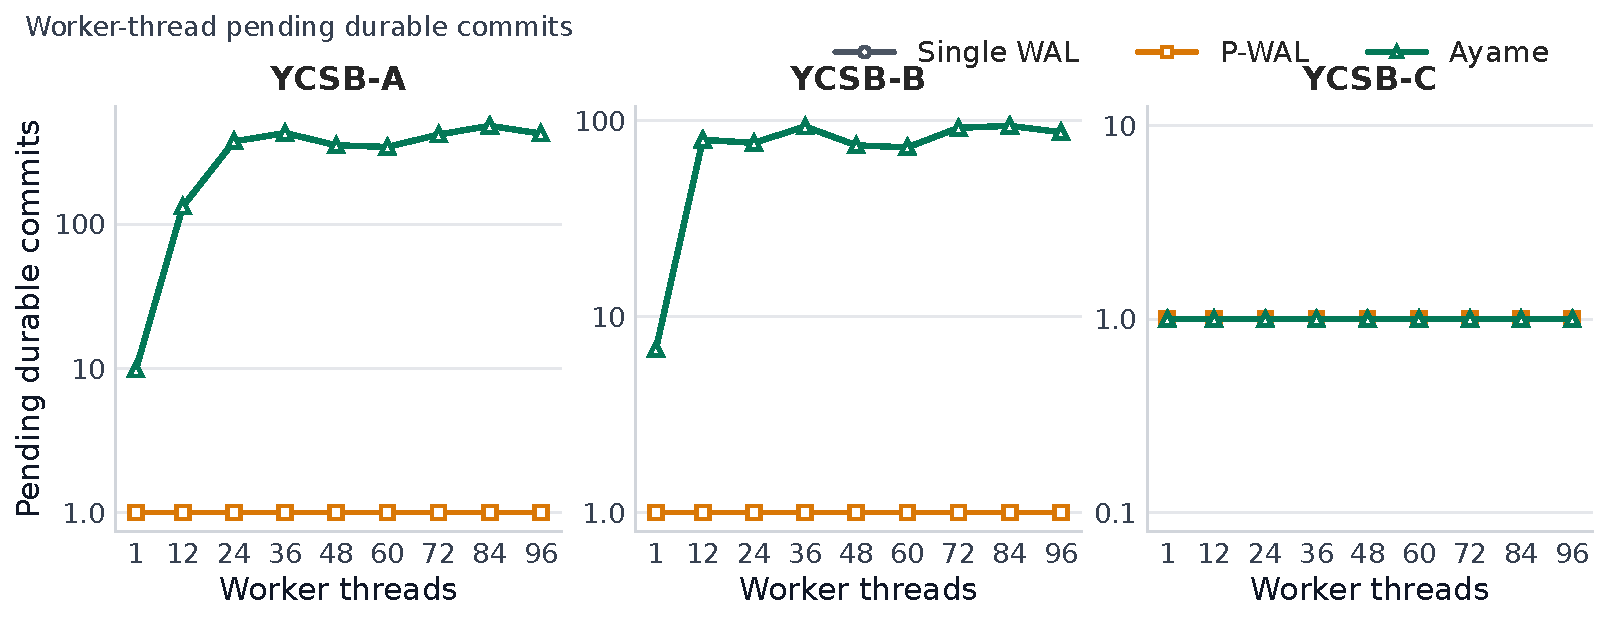
\includegraphics[width=\linewidth]{figures/fig_ycsbabc_worker_threads_pending.pdf}
  \caption{
  Pending durable commits by transaction worker threads.
  }
  \label{fig:ycsbabc-worker-pending}
\end{figure*}

\begin{figure*}[!tbp]
  \centering
  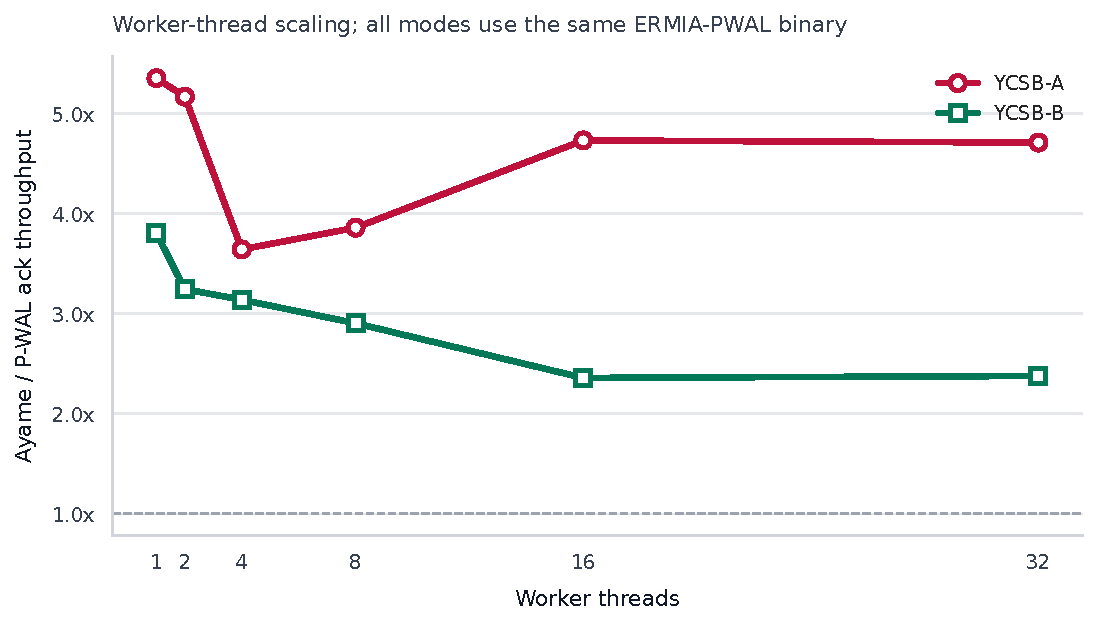
\includegraphics[width=\linewidth]{figures/fig_ycsbabc_worker_threads_ayame_speedup_vs_pwal.pdf}
  \caption{
  Ayame throughput relative to P-WAL by transaction worker threads.
  }
  \label{fig:ycsbabc-worker-speedup}
\end{figure*}

Table~\ref{tab:ycsbabc-32worker-summary} summarizes the main 32-worker
end-to-end results used in the figures.  Table~\ref{tab:ayame-speedup-32worker}
extracts the Ayame-vs-P-WAL speedups from the same measurements.

\begin{table*}[t]
  \centering
  \caption{End-to-end YCSB results at 32 transaction worker threads.}
  \label{tab:ycsbabc-32worker-summary}
  \small
  \setlength{\tabcolsep}{6pt}
  \begin{tabular}{llrrrrrrr}
    \hline
    Workload & System & Ack tps & p99 $\mu$s & Pending & fdatasync & Tx/sync & Frontier B/tx & WAL atomic/tx \\
    \hline
    YCSB-A & Single WAL & 8.6K & 4,096 & 0 & 43,222 & 1.0 & 0.0 & 6.00 \\
    YCSB-A & P-WAL & 54.1K & 512 & 0 & 270,064 & 1.0 & 0.0 & 6.00 \\
    YCSB-A & Ayame & 253.3K & 2,048 & 201 & 88,446 & 14.3 & 56.0 & 0.00 \\
    YCSB-B & Single WAL & 24.4K & 2,048 & 0 & 48,911 & 2.5 & 0.0 & 0.90 \\
    YCSB-B & P-WAL & 195.4K & 256 & 0 & 392,489 & 2.5 & 0.0 & 0.90 \\
    YCSB-B & Ayame & 470.1K & 512 & 68 & 127,491 & 18.5 & 56.0 & 0.00 \\
    YCSB-C & Single WAL & 656.2K & 48 & 0 & 0 & 0.0 & 0.0 & 0.00 \\
    YCSB-C & P-WAL & 649.4K & 49 & 0 & 0 & 0.0 & 0.0 & 0.00 \\
    YCSB-C & Ayame & 650.4K & 49 & 0 & 0 & 0.0 & 56.0 & 0.00 \\
    \hline
  \end{tabular}
  \\[-1mm]
  {\footnotesize Ack tps is durable-acknowledgment throughput. Ayame uses 7 flusher threads and 1 committer thread at 32 workers.}
\end{table*}


\begin{table*}[t]
  \centering
  \caption{Ayame throughput relative to P-WAL at 32 transaction worker threads.}
  \label{tab:ayame-speedup-32worker}
  \small
  \setlength{\tabcolsep}{6pt}
  \begin{tabular}{lrrrrr}
    \hline
    Workload & P-WAL tps & Ayame tps & Speedup & Ayame p99 $\mu$s & Ayame pending \\
    \hline
    YCSB-A & 57.9K & 253.0K & 4.37$\times$ & 16,384 & 1,657 \\
    YCSB-B & 199.9K & 442.4K & 2.21$\times$ & 512 & 75 \\
    YCSB-C & 711.6K & 680.4K & 0.96$\times$ & 49 & 0 \\
    \hline
  \end{tabular}
\end{table*}


\subsection{Why Dependency-Closed Acknowledgment Helps}
\label{sec:why-dep}

The results above reflect several mechanisms at once.  To isolate the
contribution of the dependency-closed acknowledgment rule
(\textbf{A3}) from batching and from the synchronous-versus-asynchronous
distinction, we run an ablation in which both variants use the
\emph{same} asynchronous pipeline---identical per-shard flushers and one
committer---and differ only in the acknowledgment condition.  One variant
acknowledges a transaction once the global durable prefix passes its LSN
(the global-prefix rule used by P-WAL); the other acknowledges once the
shard positions in the transaction's dependency frontier are durable
(Ayame's rule).

Figure~\ref{fig:ack-policy-ablation} and Table~\ref{tab:ack-policy}
report the result.  With only one or two flusher threads (4 and 8
workers) both rules saturate the backpressure bound, because the pipeline
itself cannot drain.  Once enough flusher threads are provisioned (16 and
32 workers), the dependency-frontier rule drains the backlog and keeps
the pending count and tail latency low, whereas the global-prefix rule
stays saturated at every worker count.  At 32 workers on YCSB-A the
global-prefix rule holds about 65{,}000 pending commits with a 131\,ms
p99 acknowledgment latency, while the dependency-frontier rule holds
about 800 pending commits with a 2\,ms p99---about two orders of
magnitude lower on both metrics, at comparable throughput.

The cause is the over-waiting of the global prefix described in
Section~\ref{sec:background}.  The global durable prefix advances only as
fast as the momentarily slowest shard, so with several shards there is
almost always one shard holding the prefix back and the backlog never
drains.  No injected straggler is required; the natural variation in
flush timing across shards is enough.  The dependency-frontier rule
acknowledges a transaction as soon as the specific shards in its frontier
are durable, so an unrelated lagging shard does not delay it.  This is
the concrete benefit of dependency-closed acknowledgment.

\begin{figure*}[!tbp]
  \centering
  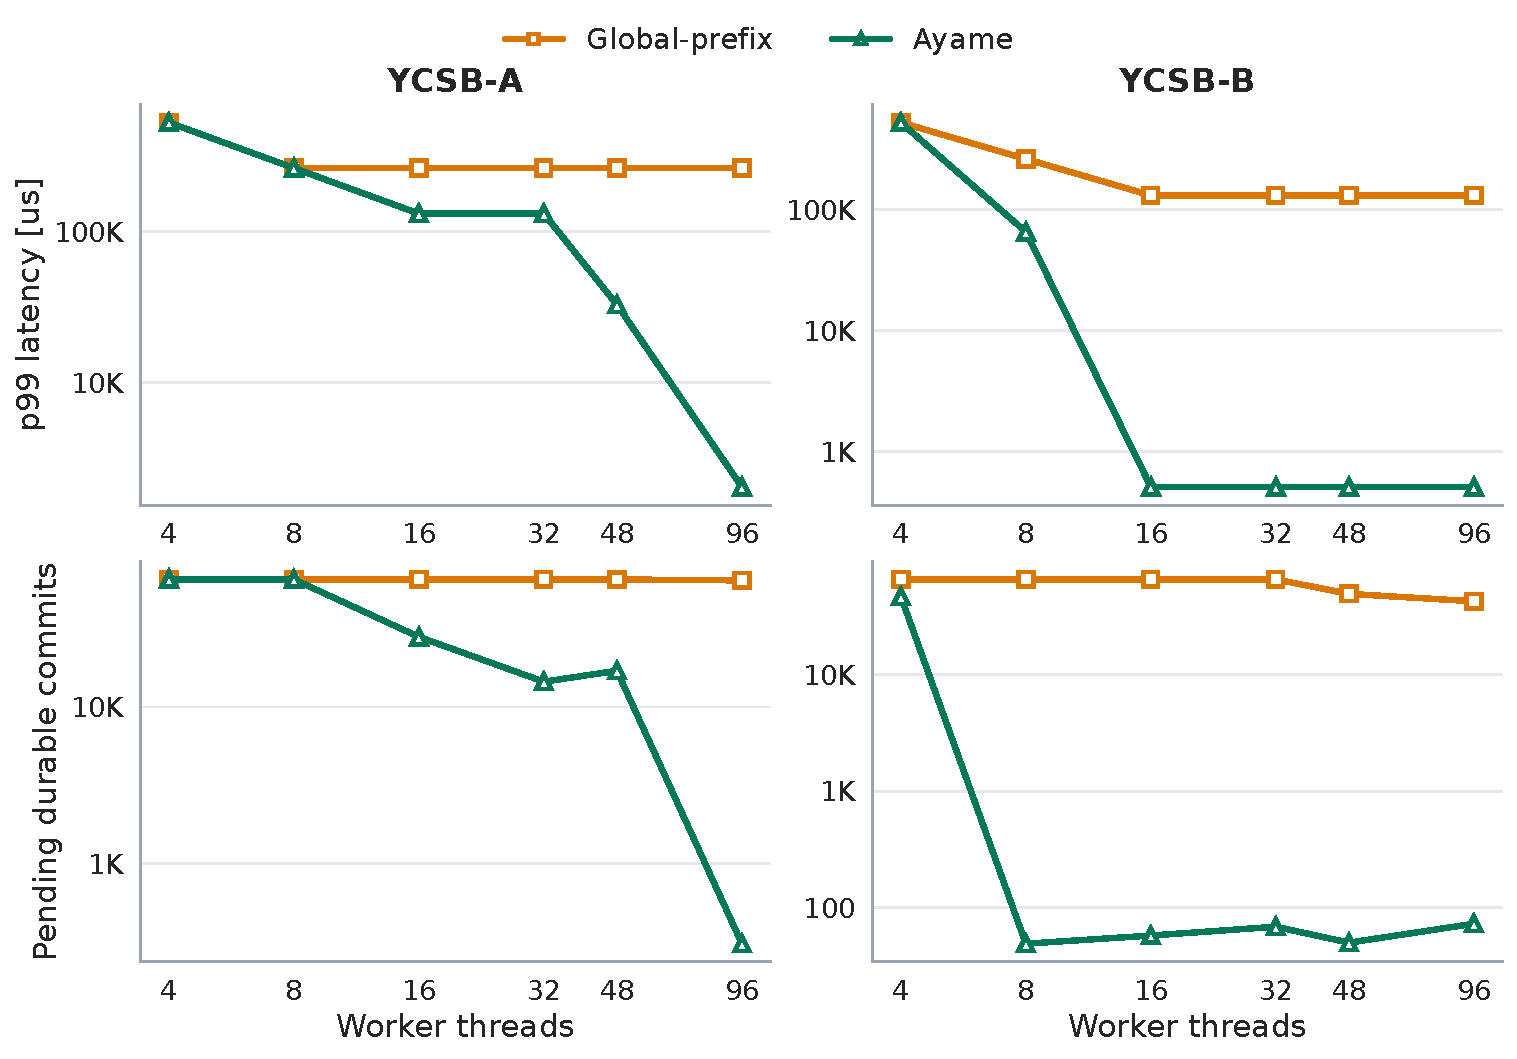
\includegraphics[width=\linewidth]{figures/fig_ack_policy_ablation.pdf}
  \caption{
  Acknowledgment-policy ablation.  Both variants use the same asynchronous
  WAL pipeline and differ only in the acknowledgment condition.  The
  global-prefix rule keeps the pending count and p99 acknowledgment
  latency saturated, while the dependency-frontier rule drains them once
  enough flusher threads are provisioned.
  }
  \label{fig:ack-policy-ablation}
\end{figure*}

\begin{table}[t]
  \centering
  \caption{Acknowledgment-policy comparison at 48 worker threads.  Both policies use the same asynchronous pipeline and differ only in the acknowledgment condition.}
  \label{tab:ack-policy}
  \small
  \begin{tabular}{llrrr}
    \hline
    Workload & Ack policy & Ack tps & p99 $\mu$s & Pending \\
    \hline
    YCSB-A & Global-prefix & 443.6K & 131,072 & 64,197 \\
    YCSB-A & Dep.\ frontier (Ayame) & 251.2K & 2,048 & 455 \\
    YCSB-B & Global-prefix & 496.6K & 2,048 & 519 \\
    YCSB-B & Dep.\ frontier (Ayame) & 452.7K & 512 & 94 \\
    \hline
  \end{tabular}
\end{table}


\subsection{Hardware Counters and Overhead}
\label{sec:overhead}

Table~\ref{tab:perf-stat-32worker} summarizes the 32-worker perf-stat analysis.
Table~\ref{tab:ycsbb-perf-scaling} shows the worker-scaling perf-stat data for
YCSB-B, where Ayame's throughput improvement is most visible.

\begin{table}[t]
  \centering
  \caption{Perf-stat summary at 32 transaction worker threads.}
  \label{tab:perf-stat-32worker}
  \small
  \begin{tabular}{llrrrrrrr}
    \hline
    Workload & System & Ack tps & CPU cores & Cycles/tx & Instr/tx & IPC & Ctx sw. & Tx/sync \\
    \hline
    YCSB-A & Single WAL & 8.1K & 1.2 & 358593 & 661657 & 1.84 & 131944 & 1.0 \\
    YCSB-A & P-WAL & 54.2K & 15.3 & 712565 & 407350 & 0.57 & 1545781 & 1.0 \\
    YCSB-A & Ayame & 245.3K & 21.3 & 215653 & 139650 & 0.65 & 3406628 & 14.3 \\
    YCSB-B & Single WAL & 22.2K & 1.0 & 115584 & 160772 & 1.39 & 139201 & 2.5 \\
    YCSB-B & P-WAL & 199.6K & 14.3 & 181391 & 102440 & 0.56 & 1448383 & 2.5 \\
    YCSB-B & Ayame & 455.0K & 25.4 & 140313 & 63232 & 0.45 & 2830611 & 17.9 \\
    YCSB-C & Single WAL & 654.4K & 32.3 & 127980 & 29559 & 0.23 & 3420 & 0.0 \\
    YCSB-C & P-WAL & 648.1K & 32.3 & 129152 & 29967 & 0.23 & 3614 & 0.0 \\
    YCSB-C & Ayame & 640.5K & 32.3 & 130724 & 33257 & 0.25 & 34983 & 0.0 \\
    \hline
  \end{tabular}
\end{table}


\begin{table}[t]
  \centering
  \caption{YCSB-B perf-stat worker scaling.}
  \label{tab:ycsbb-perf-scaling}
  \small
  \begin{tabular}{rrrrrrr}
    \hline
    Workers & Single tps & P-WAL tps & Ayame tps & Single CPU & P-WAL CPU & Ayame CPU \\
    \hline
    1 & 27.9K & 28.8K & 121.3K & 0.5 & 0.5 & 1.6 \\
    2 & 32.3K & 53.7K & 198.5K & 0.6 & 0.9 & 2.9 \\
    4 & 32.1K & 94.2K & 324.5K & 0.6 & 1.8 & 5.5 \\
    8 & 32.0K & 160.4K & 434.9K & 0.6 & 3.8 & 10.5 \\
    16 & 28.9K & 208.9K & 505.0K & 0.7 & 8.7 & 19.7 \\
    32 & 29.1K & 245.5K & 573.0K & 1.0 & 18.0 & 32.1 \\
    \hline
  \end{tabular}
\end{table}


\begin{figure}[!tbp]
  \centering
  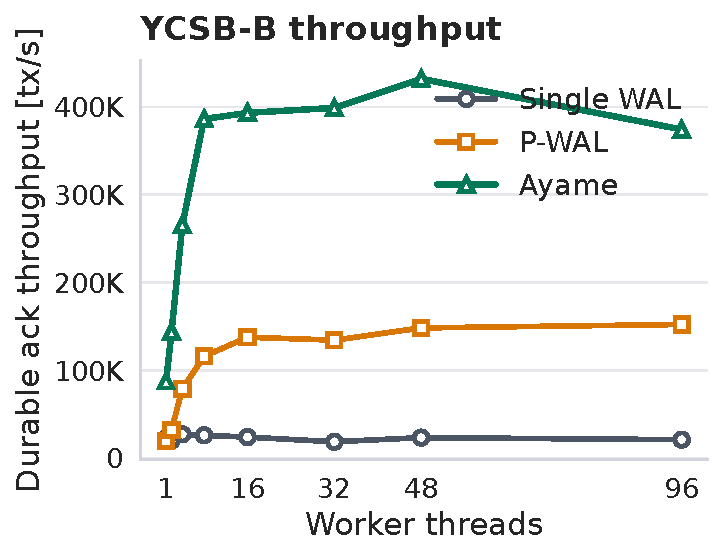
\includegraphics[width=0.86\linewidth]{figures/fig_ycsbb_perf_scaling_tps.pdf}
  \caption{
  YCSB-B durable-acknowledgment throughput in the perf-stat worker-scaling runs.
  }
  \label{fig:ycsbb-perf-scaling-tps}
\end{figure}

\begin{figure}[!tbp]
  \centering
  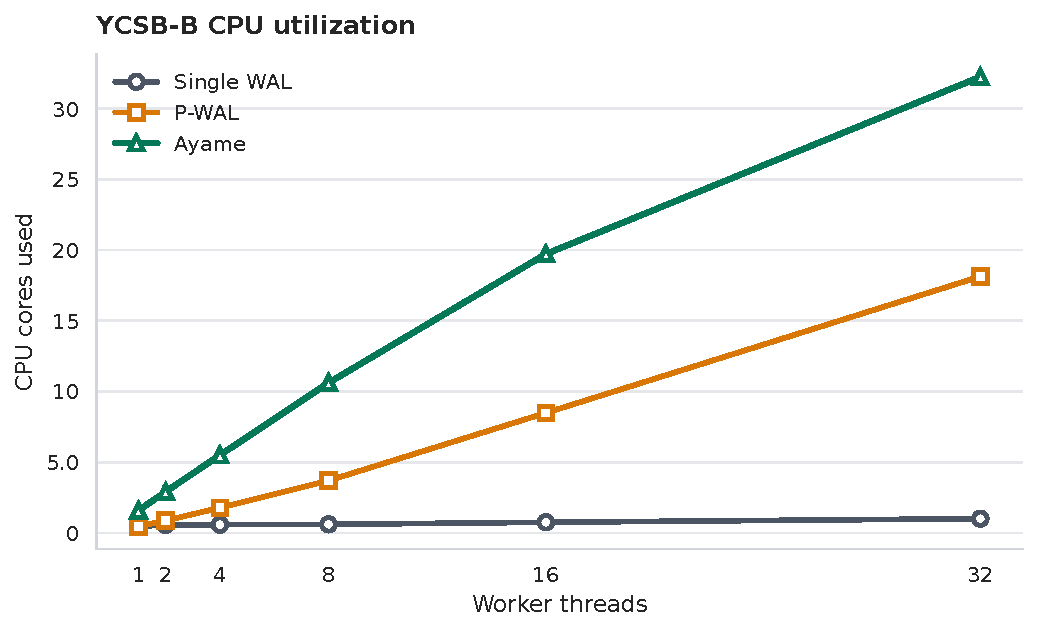
\includegraphics[width=0.86\linewidth]{figures/fig_ycsbb_perf_scaling_cpu_cores.pdf}
  \caption{
  CPU-core utilization in the YCSB-B perf-stat worker-scaling runs.
  }
  \label{fig:ycsbb-perf-scaling-cpu-cores}
\end{figure}

\begin{figure}[!tbp]
  \centering
  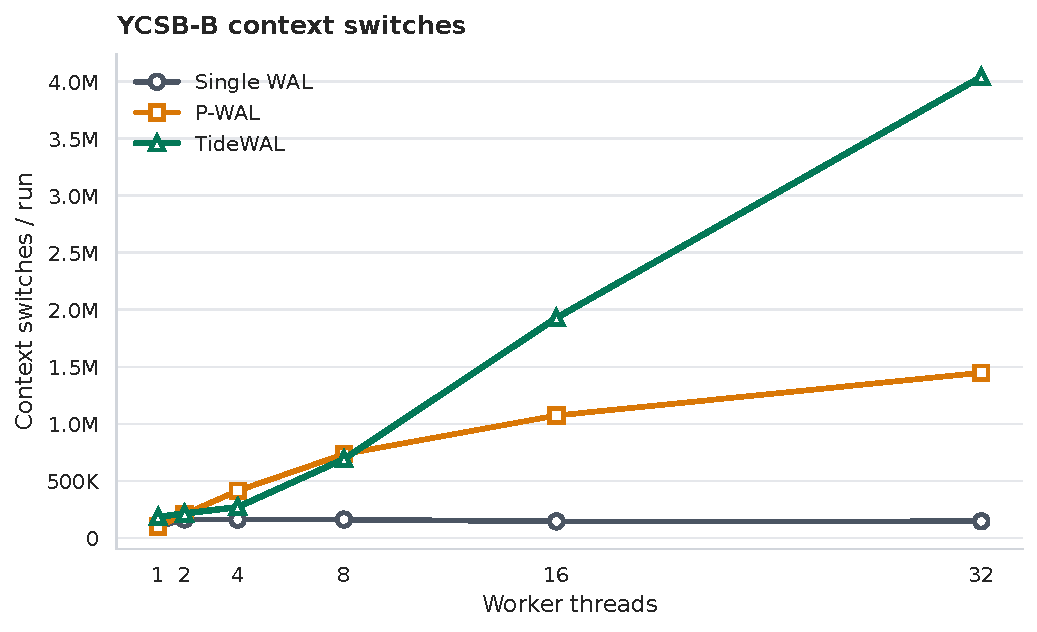
\includegraphics[width=0.86\linewidth]{figures/fig_ycsbb_perf_scaling_context_switches.pdf}
  \caption{
  Context-switch counts in the YCSB-B perf-stat worker-scaling runs.
  }
  \label{fig:ycsbb-perf-scaling-context-switches}
\end{figure}

\begin{figure*}[!tbp]
  \centering
  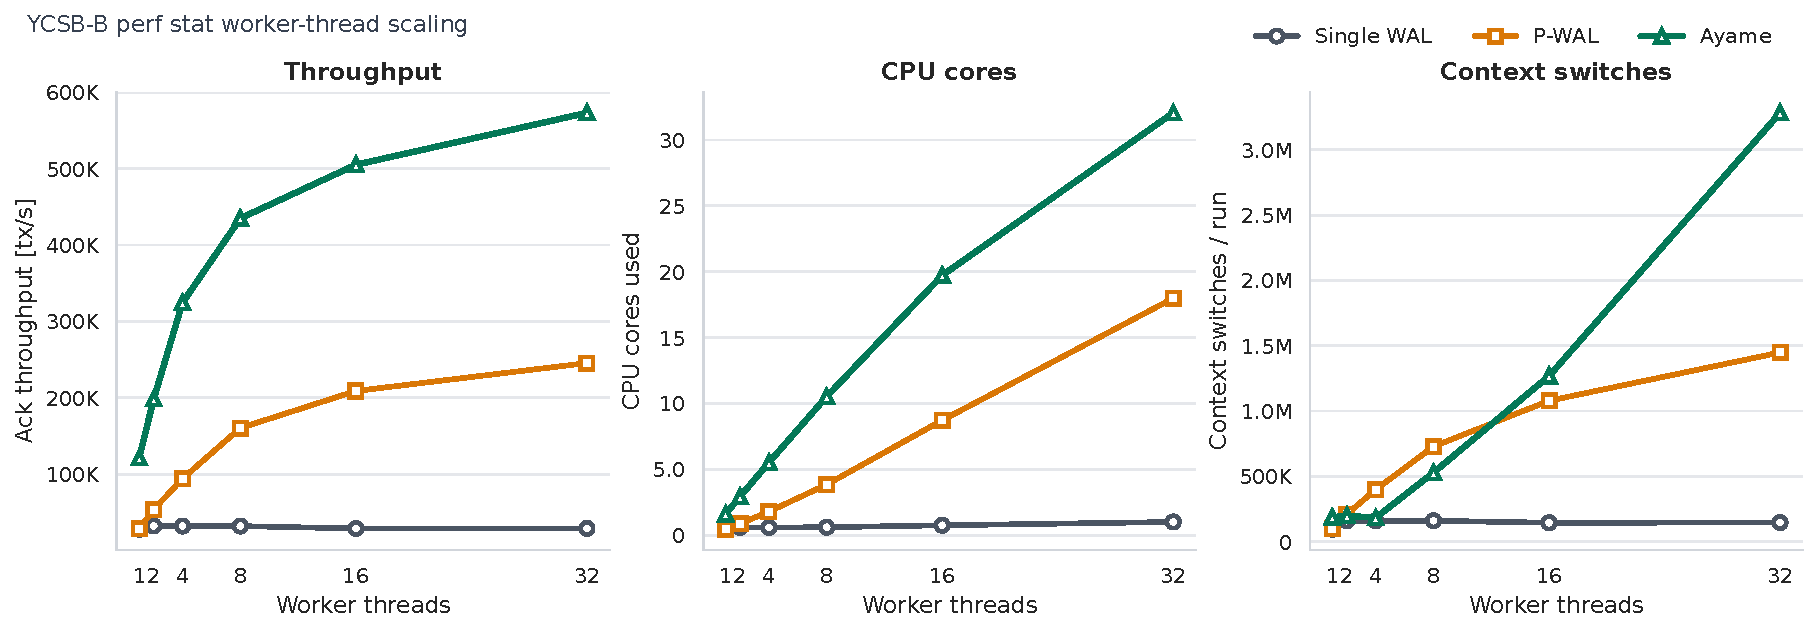
\includegraphics[width=\linewidth]{figures/fig_ycsbb_perf_scaling_perf_stat.pdf}
  \caption{
  Perf-stat summary for YCSB-B worker scaling.
  }
  \label{fig:ycsbb-perf-scaling-perf-stat}
\end{figure*}

Finally, Table~\ref{tab:ycsbc-perf-top} reports the top self-time symbols for
YCSB-C.  Since YCSB-C is read-only, this table is used as a sanity check that
the remaining cost is read-path bookkeeping rather than WAL persistence.

\begin{table*}[t]
  \centering
  \caption{Top self-time symbols for YCSB-C at 32 transaction worker threads.}
  \label{tab:ycsbc-perf-top}
  \small
  \setlength{\tabcolsep}{6pt}
  \begin{tabular}{llrl}
    \hline
    System & Rank & Self \% & Symbol \\
    \hline
    Single WAL & 1 & 58.81 & \texttt{TxExecutor::read} \\
    Single WAL & 2 & 24.00 & \texttt{TxExecutor::ssn\_parallel\_commit} \\
    Single WAL & 3 & 4.41 & \texttt{MasstreeWrapper::get\_value} \\
    Single WAL & 4 & 3.31 & \texttt{TxExecutor::mainte} \\
    Single WAL & 5 & 3.02 & \texttt{TxExecutor::read\_internal} \\
    P-WAL & 1 & 58.62 & \texttt{TxExecutor::read} \\
    P-WAL & 2 & 23.52 & \texttt{TxExecutor::ssn\_parallel\_commit} \\
    P-WAL & 3 & 4.39 & \texttt{MasstreeWrapper::get\_value} \\
    P-WAL & 4 & 3.54 & \texttt{TxExecutor::mainte} \\
    P-WAL & 5 & 3.37 & \texttt{TxExecutor::read\_internal} \\
    Ayame & 1 & 57.20 & \texttt{TxExecutor::read} \\
    Ayame & 2 & 22.58 & \texttt{TxExecutor::ssn\_parallel\_commit} \\
    Ayame & 3 & 3.87 & \texttt{MasstreeWrapper::get\_value} \\
    Ayame & 4 & 3.13 & \texttt{TxExecutor::mainte} \\
    Ayame & 5 & 3.06 & \texttt{TxExecutor::read\_internal} \\
    \hline
  \end{tabular}
  \\[-1mm]
  {\footnotesize YCSB-C is read-only; WAL bytes and fdatasync counts are zero for all systems.}
\end{table*}


\begin{figure*}[!tbp]
  \centering
  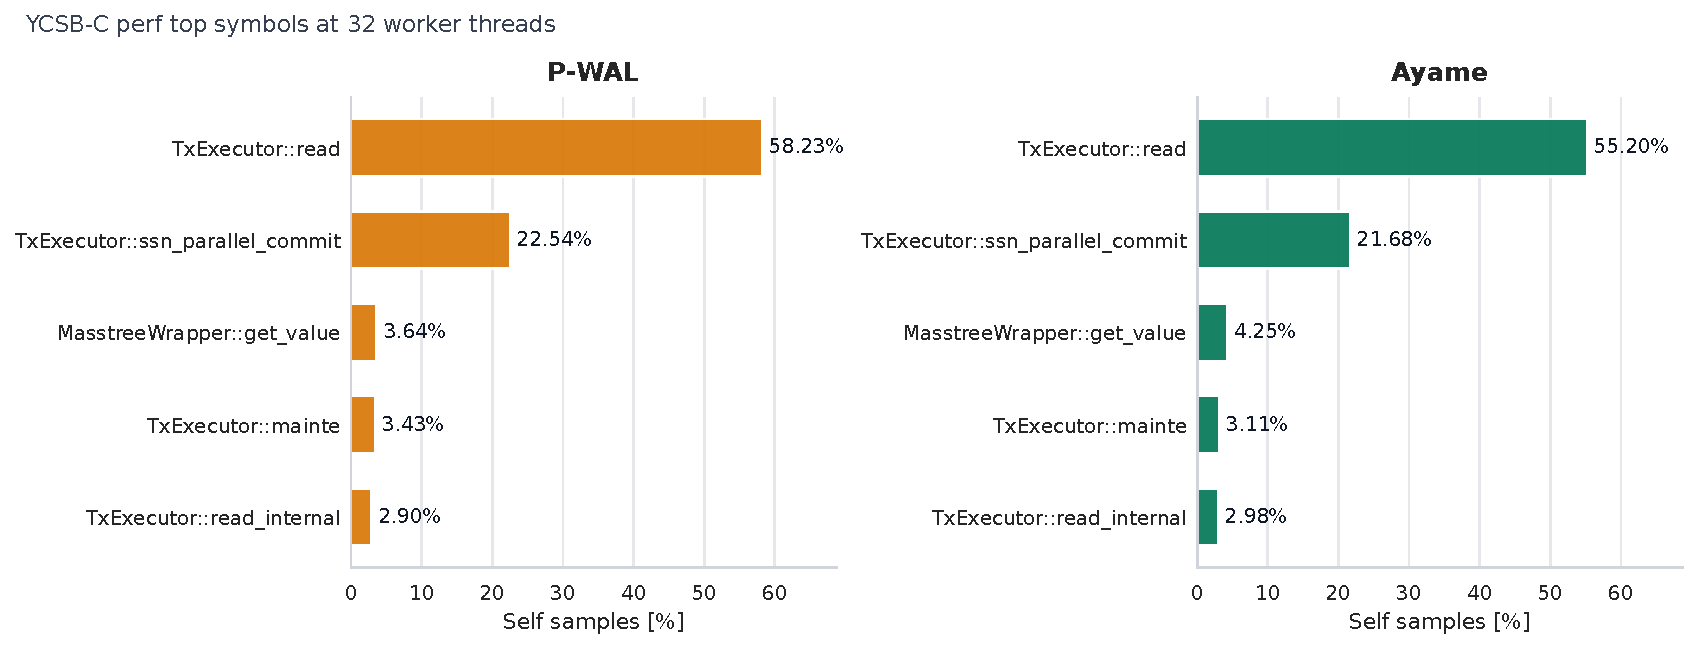
\includegraphics[width=\linewidth]{figures/fig_ycsbc_perf_top_symbols_horizontal.pdf}
  \caption{
  Top self-time symbols for YCSB-C at 32 transaction worker threads.
  }
  \label{fig:ycsbc-perf-top-symbols}
\end{figure*}
